\section{Bewertungsgrundsätze und –vorschriften}

\textbf{Bewertungsgrundsätze}:
\begin{itemize}
	\item \textbf{Grundsatz der Bilanzidentität}: Wertansätze in der Eröffnungsbilanz müssen mit denen der Schlussbilanz des vorhergehenden Geschäftsjahres übereinstimmen
	\item \textbf{Grundsatz der Unternehmensfortführung}: Annahme der Fortführung der Unternehmenstätigkeit
	\item \textbf{Stichtagsprinzip}: Vermögensgegenstände und Schulden sind zum Abschlussstichtag zu bewerten. 
	\begin{itemize}
		\item \textbf{Wertaufhellung}: Zum Abschlussstichtag bestehende Verhältnisse, die nach dem Abschlussstichtag, aber vor Aufstellung des Jahresabschlusses bekannt werden, sind auch zu berücksichtigen!
		\item \textbf{Wertbegründende Ereignisse}, die nach dem Abschlussstichtag eingetreten sind und die zu neuen, wertverändernden Verhältnissen führen, sind nicht zu berücksichtigen!
	\end{itemize}
	\item \textbf{Grundsatz der Einzelbewertung}: Vermögensgegenstände und Schulden sind einzeln zu
	bewerten
	\item \textbf{Grundsatz der Vorsicht}: Alle vorhersehbaren Risiken und Verluste berücksichtigen und Gewinne nur, wenn sie m Abschlussstichtag realisiert sind.
	\item \textbf{Grundsatz der Periodenabgrenzung}: Aufwendungen und Erträge sind unabhängig von den Zeitpunkten der Zahlungen zu berücksichtigen.
	\item \textbf{Grundsatz der Bewertungsstetigkeit}: Die auf den vorhergehenden Jahresabschluss angewandten Bewertungsmethoden sind beizubehalten.
\end{itemize}

\textbf{Vorgehen bei der Bewertung von Vermögensgegenständen und Schulden}
\begin{itemize}
	\item \textbf{Zugangsbewertung}: Wertansatz von Bilanzpositionen zum Zeitpunkt der Ersterfassung bestimmen. $\rightarrow$ \textbf{Ausgangswerte}
	\item \textbf{Folgebewertung}: Wertansätze werden fortgeführt und am Ende der Abrechnungsperiode zur Überprüfung speziellen Korrekturwerten gegenübergestellt. \\
	$\rightarrow$ \textbf{fortgeführte Ausgangswerte}
\end{itemize}
\bigskip
\textbf{Bewertungsvorschriften}: \textbf{Wertmaßstäbe} für die Zugangsbewertung:
\begin{itemize}
	\item \textbf{Anschaffungskosten} für Vermögensgegenstände = Anschaffungspreis $-$ Anschaffungskostenminderungen $+$ Anschaffungsnebenkosten $+$ Nachträgliche Anschaffungskosten (nur \textbf{Nettopreise}, excl. MwSt.)
	\item \textbf{Herstellungskosten} = Materialeinzel- und Gemeinkosten $+$ Fertigungseinzel- und Gemeinkosten $+$ Sondereinzelkosten der Fertigung $+$ Verwaltungsgemeinkosten (Wahl) $+$ Fremdkapitalkosten (Wahl) $\rightarrow$ \textbf{Sachliche Abgrenzung}
	\begin{itemize}
		\item Bei Einbeziehung von Gemeinkosten: \textbf{Grundsatz der Angemessenheit}, das angemessene Teile der Materialgemeinkosten, Fertigungsgemeinkosten des Wertverzehrs der Fertigungsanlagen betrifft. Verbietet Einbeziehung von \textbf{Unterbeschäftigungskosten}.
		\item Ausschließlich Verfahren der \textbf{Vollkostenbewertung}
		\item Bei immateriellen Vermögensgegenständen werden die bei dessen Entwicklung anfallenden
		Aufwendungen berücksichtigt
		\item \textbf{Wertuntergrenze} = Summe der Pflichtbestandteile\\
		\textbf{Wertobergrenze} = Summe der Pflicht- und Wahlbestandteile\\
		$\rightarrow$ \textbf{bilanzpolitischer Spielraum} bei Ermittlung der Herstellungskosten
	\end{itemize}
	\item \textbf{Erfüllungsbetrag} für Verbindlichkeiten und Rückstellungen: Betrag, welcher zur Erfüllung der Verpflichtung aufgewendet werden muss.\\
	Ansätze für Erfüllungsbetrag bei Verbindlichkeiten:
	\begin{itemize}
		\item \textbf{Nennbetrag} im Fall von Geldleistungsverpflichtungen
		\item \textbf{Voraussichtlich aufzuwendende Geldbetrag} im Fall von Sachleistungsverpflichtungen
		\item Rückstellungen mit Restlaufzeit $>$ 1 Jahr mit Barwert ansetzen
	\end{itemize}
	\item \textbf{Beizulegender Zeitwert}: entspricht grundsätzlich dem \textbf{Marktpreis}
	\begin{itemize}
		\item \textbf{Beschaffungsmarkt} für Vermögensgegenstände und fertige Erzeugnisse
		\item \textbf{Absatzmarkt} für unfertige und fertige Erzeugnisse
		\item Berücksichtigung des niedrigeren Werts auf Beschaffungs- und 
		\item \textbf{Funktion}: Wertansatz/Korrektur für spezifische Vermögensgegenstände und bestimmte Schulden im Rahmen der \textbf{Zugangs- und Folgebewertung}
	\end{itemize}
\end{itemize}

\textbf{Vorschriften zur Folgebewertung}:
\begin{itemize}
	\item Abnutzbare Vermögensgegenstände des AV sind planmäßig abzuschreiben
	\item Außerplanmäßige Abschreibung bei dauerhafte Wertminderung
	\item \textbf{Wertaufholungsgebot}, wenn Grund für außerplanmäßige Abschreibung entfällt
	\item Abschreibungen auf Vermögensgegenstände des UV erfolgen auf bestimmte Korrekturwerte 
	\item \textbf{Strenges Niederstwertprinzip} im UV: Abschreibungspflicht auf niedrigeren Wert, auch wenn Wertminderung dauerhaft
	\item \textbf{Gemildertes Niederstwertprinzip} im AV: Abschreibungspflicht auf niedrigeren Wert, wenn Wertminderung dauerhaft ist\\
	$\rightarrow$ Kontrolle mit \textbf{Niederstwerttest}
	\item Währungen mittels des \textbf{Devisenkassamittelkurses} umrechnen
\end{itemize}
\bigskip
\textbf{Bilanzpolitische Maßnahmen}:
\begin{center}
	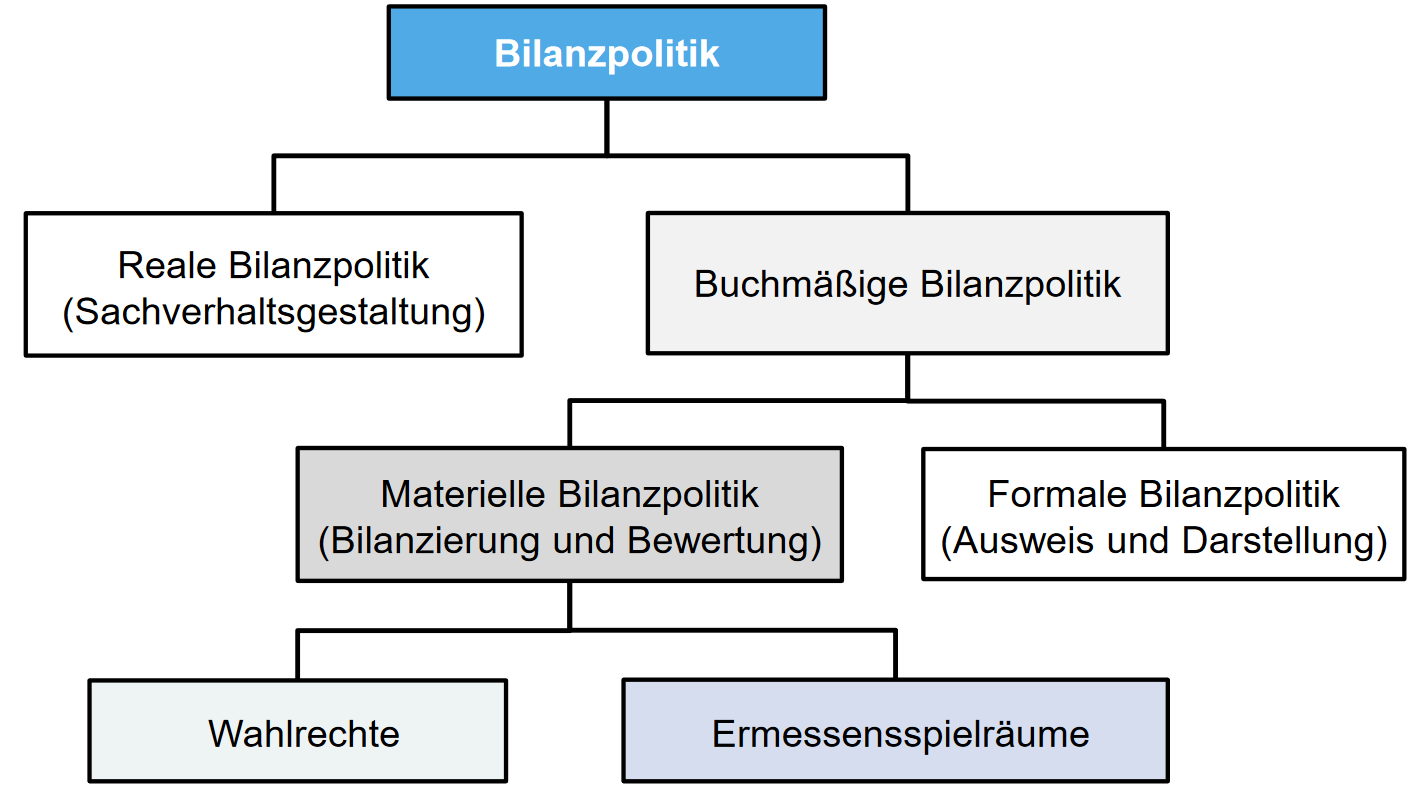
\includegraphics[width=0.7\textwidth]{images/bp.png}
\end{center}
\begin{itemize}
	\item \textbf{Bilanzansatzwahlrechte}: Disagio, Aktive latente Steuern, Selbstgeschaffene immatrielle Vermögensgegenstände des AV
	\item \textbf{Bewertungswahlrechte}: Umfang der Herstellungskosten allgemein und bei langfristiger Fertigung, Bewertungsvereinfachungsverfahren
	\item \textbf{Individualspielräume}: Bewertung von Rückstellungen, Schätzung der Nutzungsdauer von Anlagen und des Restwertes
	\item \textbf{Verfahrensspielräume}: Abschreibungsverfahren, Verfahren zur Verrechnung der Gemeinkosten, Bewertungsverfahren zur Ermittlung eines Korrekturwerts
\end{itemize}